% Documento en LaTeX con TikZ/PGF sobre la demografía de Colombia y su relación con la economía
\documentclass{article}
\usepackage{tikz}
\usepackage{pgfplots}
\pgfplotsset{compat=1.18}

\title{Evolución Demográfica de Colombia y su Relación con la Economía}
\author{Sebasg.code}
\date{\today}

\begin{document}

\maketitle

\section{Introducción}

Colombia ha experimentado importantes cambios demográficos en las últimas décadas. Desde el crecimiento de la población hasta la migración interna y externa, estos cambios han tenido un impacto significativo en la estructura económica del país. Este documento explora cómo la evolución de la demografía se relaciona con el desarrollo económico.

\section{Evolución de la Población}

En la segunda mitad del siglo XX, Colombia experimentó un rápido crecimiento poblacional debido a altas tasas de natalidad. Sin embargo, las últimas décadas han visto una desaceleración de este crecimiento, atribuida a factores como:

\begin{itemize}
    \item Mayor acceso a métodos anticonceptivos.
    \item Incremento en la educación, especialmente de mujeres.
    \item Urbanización acelerada.
\end{itemize}

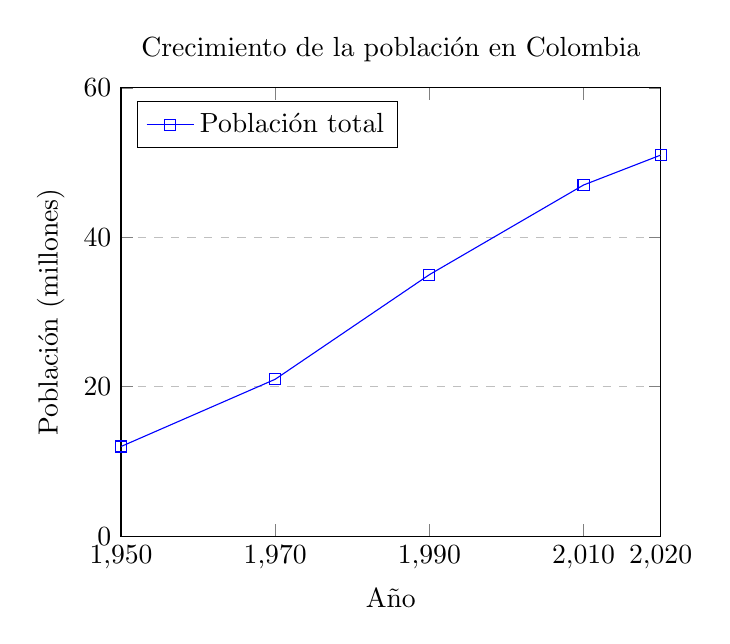
\begin{tikzpicture}
\begin{axis}[
    title={Crecimiento de la población en Colombia},
    xlabel={Año},
    ylabel={Población (millones)},
    xmin=1950, xmax=2020,
    ymin=0, ymax=60,
    xtick={1950, 1970, 1990, 2010, 2020},
    ytick={0, 20, 40, 60},
    legend pos=north west,
    ymajorgrids=true,
    grid style=dashed,
]
\addplot[
    color=blue,
    mark=square,
]
coordinates {
    (1950, 12)
    (1970, 21)
    (1990, 35)
    (2010, 47)
    (2020, 51)
};
\legend{Población total}
\end{axis}
\end{tikzpicture}

\subsection{Migración hacia las ciudades}

El fenómeno de la migración interna ha sido uno de los principales motores de la urbanización en Colombia. A continuación, se presenta una gráfica que ilustra el aumento de la población urbana en comparación con la rural:

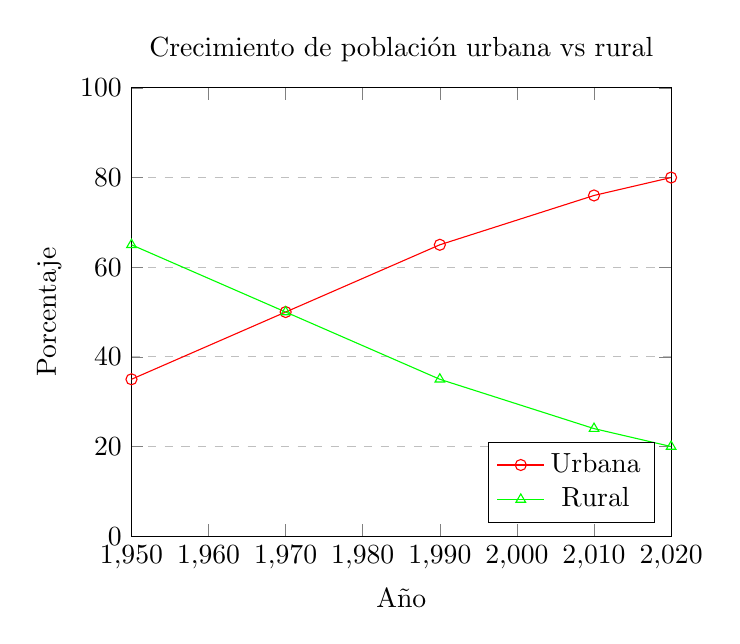
\begin{tikzpicture}
\begin{axis}[
    title={Crecimiento de población urbana vs rural},
    xlabel={Año},
    ylabel={Porcentaje},
    xmin=1950, xmax=2020,
    ymin=0, ymax=100,
    legend pos=south east,
    ymajorgrids=true,
    grid style=dashed,
]
\addplot[
    color=red,
    mark=o,
]
coordinates {
    (1950, 35)
    (1970, 50)
    (1990, 65)
    (2010, 76)
    (2020, 80)
};
\addplot[
    color=green,
    mark=triangle,
]
coordinates {
    (1950, 65)
    (1970, 50)
    (1990, 35)
    (2010, 24)
    (2020, 20)
};
\legend{Urbana, Rural}
\end{axis}
\end{tikzpicture}

\section{Factores Clave en los Cambios Demográficos}

\subsection{Aumento en la tasa de educación}

El acceso a la educación, especialmente entre las mujeres, ha cambiado significativamente la dinámica demográfica. La siguiente gráfica muestra el incremento en el porcentaje de alfabetización en el país:

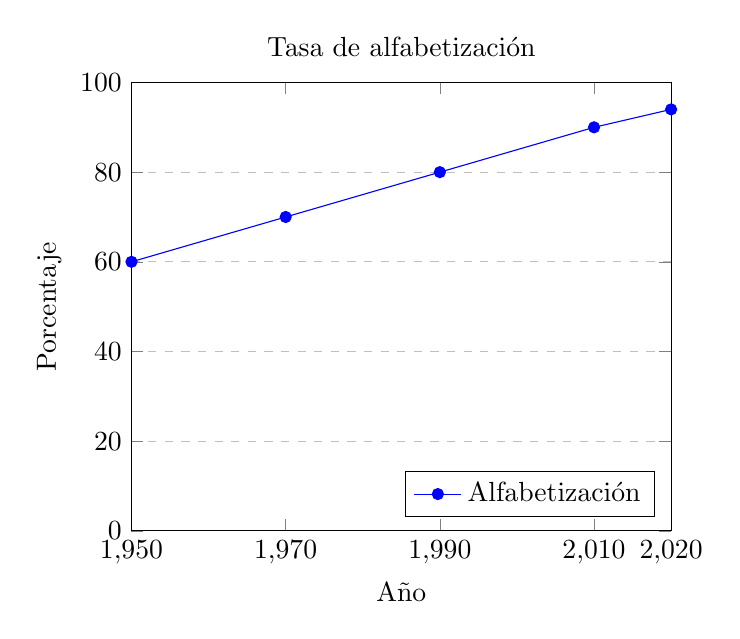
\begin{tikzpicture}
\begin{axis}[
    title={Tasa de alfabetización},
    xlabel={Año},
    ylabel={Porcentaje},
    xmin=1950, xmax=2020,
    ymin=0, ymax=100,
    xtick={1950, 1970, 1990, 2010, 2020},
    ytick={0, 20, 40, 60, 80, 100},
    legend pos=south east,
    ymajorgrids=true,
    grid style=dashed,
]
\addplot[
    color=blue,
    mark=*,
]
coordinates {
    (1950, 60)
    (1970, 70)
    (1990, 80)
    (2010, 90)
    (2020, 94)
};
\legend{Alfabetización}
\end{axis}
\end{tikzpicture}

\subsection{Reducción en la tasa de natalidad}

La tasa de natalidad ha disminuido considerablemente debido a factores como el acceso a métodos anticonceptivos y mayores niveles educativos. A continuación se muestra su evolución:

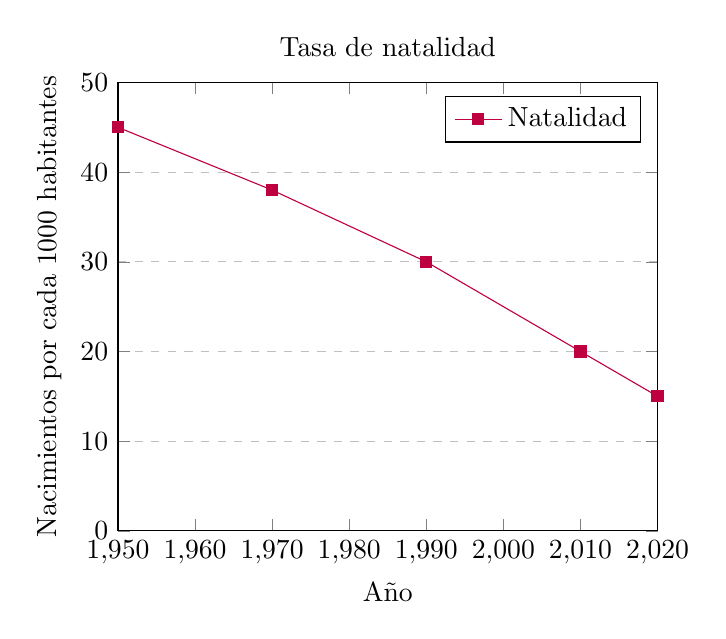
\begin{tikzpicture}
\begin{axis}[
    title={Tasa de natalidad},
    xlabel={Año},
    ylabel={Nacimientos por cada 1000 habitantes},
    xmin=1950, xmax=2020,
    ymin=0, ymax=50,
    legend pos=north east,
    ymajorgrids=true,
    grid style=dashed,
]
\addplot[
    color=purple,
    mark=square*,
]
coordinates {
    (1950, 45)
    (1970, 38)
    (1990, 30)
    (2010, 20)
    (2020, 15)
};
\legend{Natalidad}
\end{axis}
\end{tikzpicture}

\section{Relación con la Economía}

La evolución demográfica ha influido en varios aspectos económicos:

\subsection{Urbanización y Mercado Laboral}

El proceso de urbanización ha generado un cambio en la estructura del mercado laboral, con un crecimiento en sectores como:

\begin{itemize}
    \item Servicios.
    \item Industria.
    \item Comercio.
\end{itemize}

\subsection{Migración y Distribución de Recursos}

La migración interna, desde zonas rurales hacia ciudades, y la migración externa han afectado la distribución de recursos y las remesas enviadas desde el exterior.

\section{Proyección a Futuro}

Basándonos en las tendencias actuales, se puede prever que:

\begin{itemize}
    \item La urbanización alcanzará niveles cercanos al 85\% de la población total en 2030.
    \item La tasa de natalidad podría estabilizarse en valores cercanos a 12 nacimientos por cada 1000 habitantes.
    \item El aumento en la alfabetización y la educación superior continuará impulsando una transición hacia una economía basada en servicios y tecnología.
    \item La migración hacia las ciudades podría generar mayores presiones en infraestructura y servicios públicos.
\end{itemize}

\subsection{Proyección Gráfica}

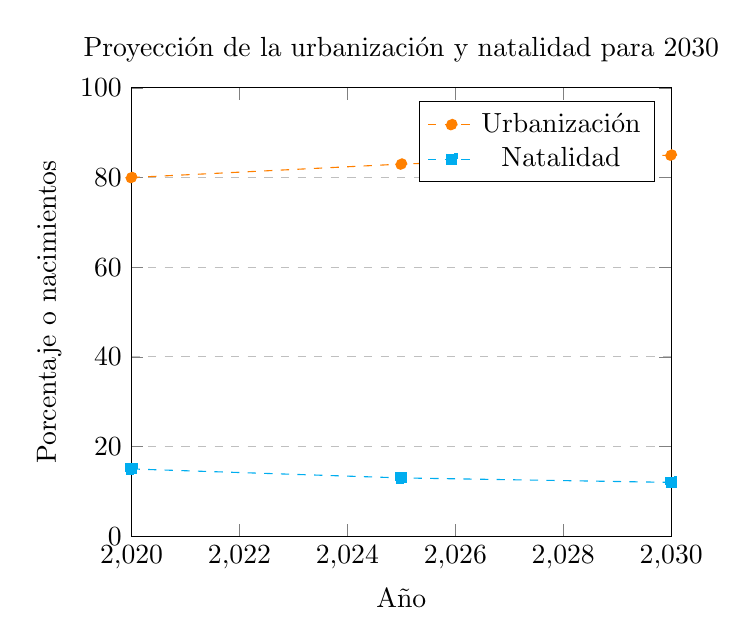
\begin{tikzpicture}
\begin{axis}[
    title={Proyección de la urbanización y natalidad para 2030},
    xlabel={Año},
    ylabel={Porcentaje o nacimientos},
    xmin=2020, xmax=2030,
    ymin=0, ymax=100,
    legend pos=north east,
    ymajorgrids=true,
    grid style=dashed,
]
\addplot[
    color=orange,
    mark=*,
    dashed
]
coordinates {
    (2020, 80)
    (2025, 83)
    (2030, 85)
};
\addplot[
    color=cyan,
    mark=square*,
    dashed
]
coordinates {
    (2020, 15)
    (2025, 13)
    (2030, 12)
};
\legend{Urbanización, Natalidad}
\end{axis}
\end{tikzpicture}

\section{Conclusión}

El vínculo entre la demografía y la economía en Colombia es evidente. Los cambios en la población han moldeado el panorama económico, y es crucial considerar estos factores en la planificación de políticas públicas para un desarrollo sostenible. Las proyecciones demográficas muestran un panorama de retos y oportunidades que demandarán adaptaciones significativas en las políticas económicas.

\end{document}
